\subsection{Sprint 7: da 2024-06-25 a 2024-07-02}
Il team in vista della RTB si appresta a concludere le attività di programmazione relative al \glossario{PoC} e nell'ultimare le sezioni incomplete dei documenti, focalizzandosi maggiormente sulla sezione documentale prima della consegna.


\subsubsection{Obiettivi}
\begin{itemize}
  \item Revisione consuntivi \PdP;
  \item Aggiunta metriche alle \NdP;
  \item Completamento sezioni incomplete \NdP;
  \item Stesura sezione test nel \PdQ;
  \item Stesura dei verbali interni;
  \item Gestione stato Utente/Tecnico a \glossario{front-end};
  \item Creazione interfaccia Chat a \glossario{front-end};
  \item Implementazione funzioni per generare il \glossario{prompt} e mostrarlo a \glossario{front-end}.
\end{itemize}

\begin{figure}[H]
  \centering
  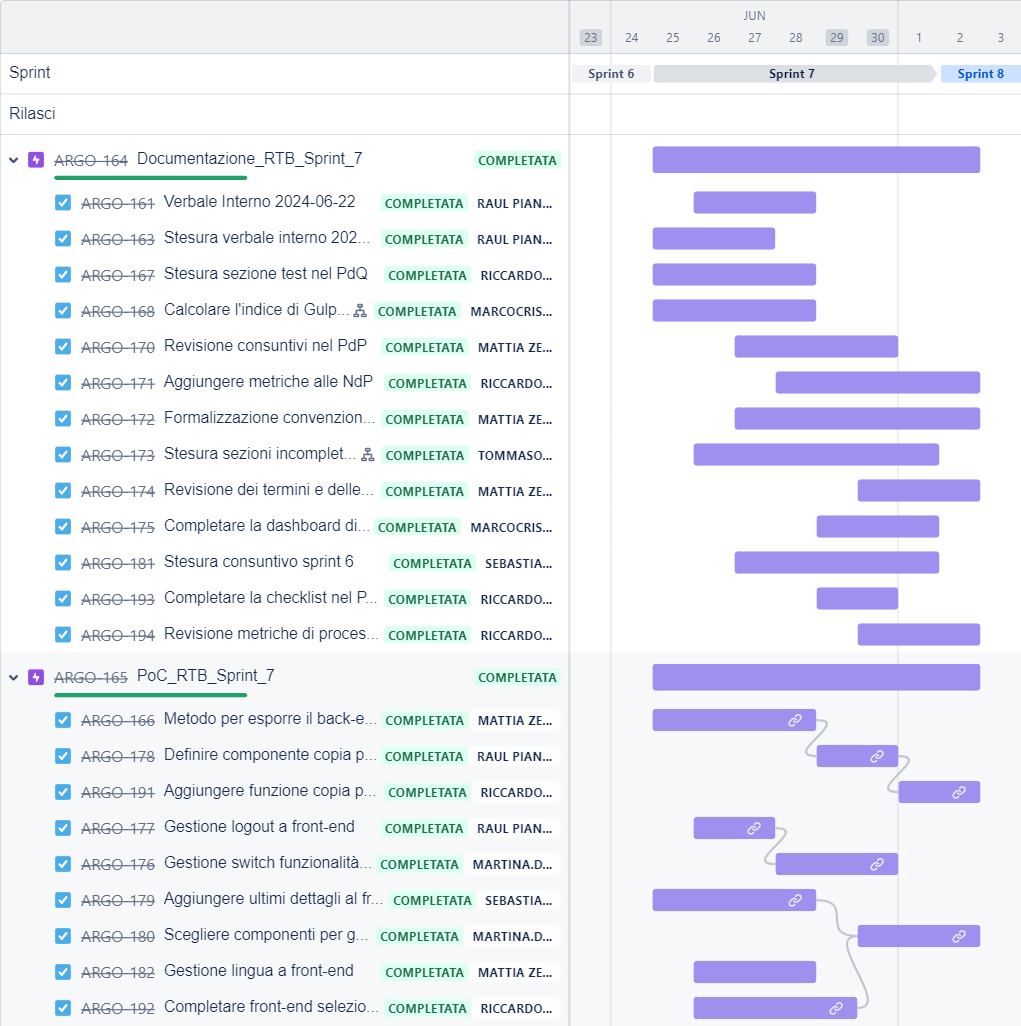
\includegraphics[width=0.90\textwidth]{assets/Pianificazione/Sprint-7/gantt.png}
  \caption{Sprint 7 - Diagramma di Gantt}\label{fig:sprint-7-gantt}
\end{figure}